\documentclass[oneside]{book}
\usepackage[utf8]{inputenc}
\usepackage[explicit, clearempty]{titlesec}
\titleformat{\chapter}[display]{\bfseries\filright}{\huge\chaptername~\thechapter}{20pt}{\Huge#1}
\titleformat{name=\chapter, numberless}[display]{\bfseries\filright}{}{0pt}{\Huge#1}[\addcontentsline{toc}{chapter}{#1}]

\usepackage[T1]{fontenc}
\usepackage{graphicx}
\usepackage[french]{babel}
\usepackage{tabu}

\title{Cahier des charges}

\author{Brahim BAHAIDA}

\date{Jeudi 17 janvier 2019}



\begin{document}

\begin{titlepage}
\maketitle
\thispagestyle{empty}
\end{titlepage}

\tableofcontents


%%%%%%%%%%%%%%%%%%%%%%%%%%%%%%%%%%%%%%%%%%%%%%%%%%%%%%%%%%%%%%%%%%%%%%%%%%%%%%%%%%%%%%%%%%%%%%%%%%%%%%%%%%%%%%%%%%%%%%%%%%%%%%%%%%%%%%
\chapter*{Introduction}

Ce document a pour objectif de décrire le contexte et les exigences du projet et, à cette fin, nous commencerons par une vision globale du projet et présenterons ensuite les spécifications du projet.

\section*{liste de diffusion}
\begin{tabu} to 0.8\textwidth { | X[c] | X[c] | }
 \hline
 \textbf{Prénom et Nom} & \textbf{Rôle} \\
 \hline
 Ghassen HAMROUNI  & Encadrant profissionnel \\
\hline
Rim KAABI  & Encadrant académique \\
\hline
Brahim BAHAIDA  & Réalisateur du projet \\
\hline

\end{tabu}

\section*{suivi des versions}

\begin{tabu} to 0.8\textwidth { | X[c] | X[c] | }
 \hline
 \textbf{Version} & \textbf{Dernière modification} \\
 \hline
 1.0  & 17/01/2019 \\
\hline
\end{tabu}

\section*{glossaire}

\begin{tabu} to 0.8\textwidth { | X[c] | X[c] | }
 \hline
 \textbf{Acronyme} & \textbf{Signification} \\
 \hline
 DQM  & Data Quality Management \\
\hline
DFD  & Data Flow Diagrams \\
\hline
DQ  & Data Quality \\
\hline
BI  & Business Intelligence \\
\hline
WCAG  & Web Content Accessibility Guidelines \\
\hline
WAI  & Web Accessibility Initiative \\
\hline
W3C  & World Wide Web Consortium \\
\hline
EF  & Exigence fonctionnelle \\
\hline

\end{tabu}
\\
\chapter{Vision globale du projet}
Ce chapitre vise à présenter le contexte, le planning et les contraintes du projet.
\section{Description du projet}

Data Quality (DQ) est un concept et un terme de business désignant la qualité des données utilisées dans un but particulier. Souvent, le terme DQ s'applique à la qualité des données utilisées dans la prise de décisions des entreprises, mais il peut aussi désigner la qualité des données utilisées dans les recherches, les campagnes, les processus et plus encore.
\\
\\
Une erreur dans un système de stockage de données ou un rapport de business intelligence peut sembler minime au premier abord. Il peut être tentant pour les analystes de l'ignorer ou de truquer les chiffres du mois. Peut-être qu'ils se diront : " Ce sera corrigé plus tard ".
\\
\\
Cependant, si l'équipe chargée du data science ou du Business Intelligence ne comprend pas parfaitement pourquoi cela s'est produit, elle risque de se retrouver avec une erreur encore plus grande dans son prochain rapport ou dans les informations qu'elle fournira à la direction.
\\
\\
L'objectif de ce projet est de concevoir et de développer une plateforme de gestion et d'amélioration de la qualité des données clients pour les institutions financières afin d'améliorer leur conformité réglementaire.
\\
\\
Nous utiliserons le diagramme de contexte de la technique DFD (Data Flow Diagrams) pour illustrer les fonctionnalités de la plate-forme. 
\\
\\

\begin{figure}[h!]
  \caption{Diagramme de contexte}
  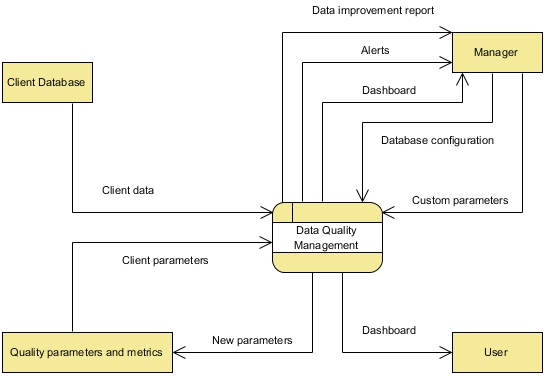
\includegraphics[width=\textwidth]{img/Context_DFD.jpg}
\end{figure}


\section{Planning}

ce projet doit être complètement achevé au plus tard le début du mois de juillet 2019.

\section{Contraintes}
Nous pouvons considérer les contraintes comme des exigences non fonctionnelles qui présentent des exigences internes pour le système et qui sont invisibles vis-à-vis de nos clients.
\subsection{Accessibilité}
Le système vise à atteindre au moins le niveau minimum d'accessibilité du Web (A) selon les niveaux d'accessibilité WCAG 2.0 établis par la WAI (Web Accessibility Initiative) du World Wide Web Consortium (W3C).
\subsection{Responsive design}
Pour rendre la plateforme conviviale, nous devons respecter les points suivants:
\begin{itemize}
    \item \textbf{Paramétrage HTML}
    \item \textbf{Mise en page flexible}
    \item \textbf{Type flexible}
    \item \textbf{Images flexibles}
\end{itemize}
\subsection{Sécurité}
Pour être conforme aux principes de sécurité, la plate-forme doit être protégée contre le top 10 des vulnérabilités web publiées par l'OWASP.

\section{Public de la plate-forme}
Cette plate-forme sera réalisée non pas pour un usage public via Internet mais au sein du réseau d'un client et pour cela elle aura trois types d'utilisateurs.\\
\\
    \begin{itemize}
        \item \textbf{Manager:} il est chargé d'ajouter et d'éditer les configurations des bases de données et des paramètres, il peut générer le rapport de qualité des données.
        \\
        \item \textbf{User:} il est un simple utilisateur qui peut accéder aux fonctionnalités de la plateforme mais il ne peut pas ajouter ou modifier les configurations.
        \\
        \item \textbf{Superuser:} Il est chargé d'ajouter de nouveaux utilisateurs et de modifier leurs rôles, mais il n'aura pas accès aux autres fonctionnalités de la plateforme pour respecter au mieux le principe du SoD.
    \end{itemize}
\chapter{Les spécifications du projet}

Ce chapitre a pour but d'illustrer toute la spécification du projet et pour cela il est divisé en deux parties, nous avons commencé par les spécifications fonctionnelles et ensuite nous avons présenté les spécifications techniques.

\section{Specifications fonctionnelles} 

Les besoins fonctionnels servent à présenter les actions que doit effectuer le
Système en réponse à une demande présentée par un utilisateur. La figure suivante illustre le diagramme de navigation proposé.
\\
\\
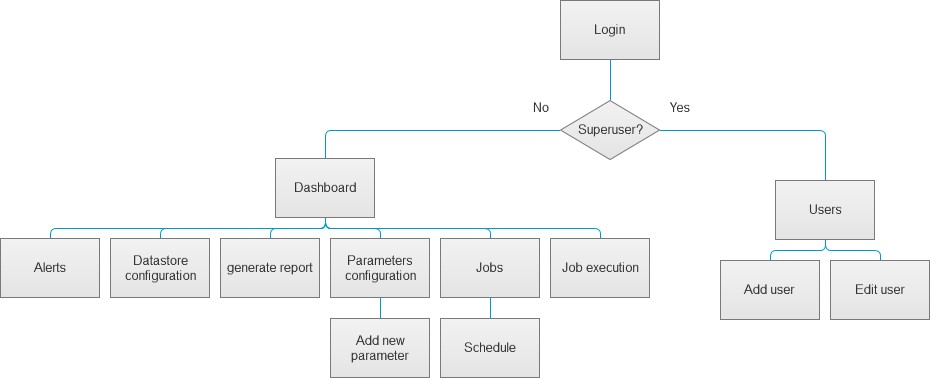
\includegraphics[width=\textwidth]{img/pages.jpg}\\
\\

A ce niveau, nous devons spécifier nos exigences en langage naturel, en utilisant les fiche GABARIT-VOLERE.
\\
\\
\noindent\fbox{%
    \parbox{\textwidth}{%
        \textbf{Numero d'exigence:} EF1
        \qquad \textbf{Type d'exigence:} Exigence fonctionnelle
         \\
        \\
        \textbf{Cas d’utilisation:} S'authentifier
        \\
        \\
        \textbf{Description :} le système doit fournir une interface pour l'authentification
        \\
        \\
        \textbf{Acteur:} Tous les utilisateurs
        \\
        \\
        \textbf{Contentement du maître d’ouvrage:} 3
        \\
        \\
        \textbf{Mécontentement du maître d’ouvrage:} 5
        \\
        \\
        \textbf{Exigences dépendantes:} 
    }%
}
\\
\\
\\
\noindent\fbox{%
    \parbox{\textwidth}{%
        \textbf{Numero d'exigence:} EF2
        \qquad \textbf{Type d'exigence:} Exigence fonctionnelle
         \\
        \\
        \textbf{Cas d’utilisation:} Ajouter un utilisateur
        \\
        \\
        \textbf{Description :} le système doit permettre au Superuser d'ajouter de nouveaux utilisateurs
        \\
        \\
        \textbf{Acteur:} Superuser
        \\
        \\
        \textbf{Contentement du maître d’ouvrage:} 3
        \\
        \\
        \textbf{Mécontentement du maître d’ouvrage:} 4
        \\
        \\
        \textbf{Exigences dépendantes:} EF1
    }%
}
\\
\\
\\
\noindent\fbox{%
    \parbox{\textwidth}{%
        \textbf{Numero d'exigence:} EF3
        \qquad \textbf{Type d'exigence:} Exigence fonctionnelle
         \\
        \\
        \textbf{Cas d’utilisation:} Modifier un utilisateur
        \\
        \\
        \textbf{Description :} le système doit permettre au Superuser de modifier les rôles des utilisateurs
        \\
        \\
        \textbf{Acteur:} Superuser
        \\
        \\
        \textbf{Contentement du maître d’ouvrage:} 3
        \\
        \\
        \textbf{Mécontentement du maître d’ouvrage:} 3
        \\
        \\
        \textbf{Exigences dépendantes:} EF1
    }%
}

\noindent\fbox{%
    \parbox{\textwidth}{%
        \textbf{Numero d'exigence:} EF4
        \qquad \textbf{Type d'exigence:} Exigence fonctionnelle
         \\
        \\
        \textbf{Cas d’utilisation:} Consulter le dashboard
        \\
        \\
        \textbf{Description :} le système doit permettre au Manger et au Simpleuser d'accéder au dashboard alimenté par les indicateurs de mesure
        \\
        \\
        \textbf{Acteur:} Manager, Simpleuser
        \\
        \\
        \textbf{Contentement du maître d’ouvrage:} 4
        \\
        \\
        \textbf{Mécontentement du maître d’ouvrage:} 4
        \\
        \\
        \textbf{Exigences dépendantes:} EF1
    }%
}
\\
\\
\\
\noindent\fbox{%
    \parbox{\textwidth}{%
        \textbf{Numero d'exigence:} EF5
        \qquad \textbf{Type d'exigence:} Exigence fonctionnelle
         \\
        \\
        \textbf{Cas d’utilisation:} Ajouter la configuration de datastores
        \\
        \\
        \textbf{Description :} le système doit permettre au Manager d'ajouter des configurations de datastores
        \\
        \\
        \textbf{Acteur:} Manager
        \\
        \\
        \textbf{Contentement du maître d’ouvrage:} 5
        \\
        \\
        \textbf{Mécontentement du maître d’ouvrage:} 5
        \\
        \\
        \textbf{Exigences dépendantes:} EF1
    }%
}
\\
\\
\\
\noindent\fbox{%
    \parbox{\textwidth}{%
        \textbf{Numero d'exigence:} EF6
        \qquad \textbf{Type d'exigence:} Exigence fonctionnelle
         \\
        \\
        \textbf{Cas d’utilisation:} Ajouter la configuration des paramètres de qualité
        \\
        \\
        \textbf{Description :} le système doit permettre au Manager d'ajouter la configuration des paramètres de qualité
        \\
        \\
        \textbf{Acteur:} Manager
        \\
        \\
        \textbf{Contentement du maître d’ouvrage:} 5
        \\
        \\
        \textbf{Mécontentement du maître d’ouvrage:} 5
        \\
        \\
        \textbf{Exigences dépendantes:} EF1
    }%
}
\noindent\fbox{%
    \parbox{\textwidth}{%
        \textbf{Numero d'exigence:} EF7
        \qquad \textbf{Type d'exigence:} Exigence fonctionnelle
         \\
        \\
        \textbf{Cas d’utilisation:} Ajouter un nouveau paramètre de qualité
        \\
        \\
        \textbf{Description :} le système doit permettre au Manger d'ajouter un nouveau paramètre de qualité
        \\
        \\
        \textbf{Acteur:} Manager
        \\
        \\
        \textbf{Contentement du maître d’ouvrage:} 4
        \\
        \\
        \textbf{Mécontentement du maître d’ouvrage:} 4
        \\
        \\
        \textbf{Exigences dépendantes:} EF1, EF6
    }%
}
\\
\\
\\
\noindent\fbox{%
    \parbox{\textwidth}{%
        \textbf{Numero d'exigence:} EF8
        \qquad \textbf{Type d'exigence:} Exigence fonctionnelle
         \\
        \\
        \textbf{Cas d’utilisation:} Ajouter des jobs
        \\
        \\
        \textbf{Description :} le système doit permettre au Manager d'ajouter des jobs
        \\
        \\
        \textbf{Acteur:} Manager
        \\
        \\
        \textbf{Contentement du maître d’ouvrage:} 5
        \\
        \\
        \textbf{Mécontentement du maître d’ouvrage:} 4
        \\
        \\
        \textbf{Exigences dépendantes:} EF1, EF5, EF6
    }%
}
\\
\\
\\
\noindent\fbox{%
    \parbox{\textwidth}{%
        \textbf{Numero d'exigence:} EF9
        \qquad \textbf{Type d'exigence:} Exigence fonctionnelle
         \\
        \\
        \textbf{Cas d’utilisation:} Ajouter la planification des jobs
        \\
        \\
        \textbf{Description :} le système doit permettre au Manager de planifier l'exécution des jobs
        \\
        \\
        \textbf{Acteur:} Manager
        \\
        \\
        \textbf{Contentement du maître d’ouvrage:} 5
        \\
        \\
        \textbf{Mécontentement du maître d’ouvrage:} 3
        \\
        \\
        \textbf{Exigences dépendantes:} EF1, EF5, EF6, EF8
    }%
}
\noindent\fbox{%
    \parbox{\textwidth}{%
        \textbf{Numero d'exigence:} EF10
        \qquad \textbf{Type d'exigence:} Exigence fonctionnelle
        \\
        \\
        \textbf{Cas d’utilisation:} Visualiser le état d'exécution d'un job
        \\
        \\
        \textbf{Description :} le système doit permettre au Manger de visualiser le état d'exécution d'un job
        \\
        \\
        \textbf{Acteur:} Manager
        \\
        \\
        \textbf{Contentement du maître d’ouvrage:} 3
        \\
        \\
        \textbf{Mécontentement du maître d’ouvrage:} 2
        \\
        \\
        \textbf{Exigences dépendantes:} EF1, EF6
    }%
}
\\
\\
\\
\noindent\fbox{%
    \parbox{\textwidth}{%
        \textbf{Numero d'exigence:} EF11
        \qquad \textbf{Type d'exigence:} Exigence fonctionnelle
         \\
        \\
        \textbf{Cas d’utilisation:} Générer un rapport
        \\
        \\
        \textbf{Description :} le système doit permettre au Manager de générer un rapport
        \\
        \\
        \textbf{Acteur:} Manager
        \\
        \\
        \textbf{Contentement du maître d’ouvrage:} 5
        \\
        \\
        \textbf{Mécontentement du maître d’ouvrage:} 5
        \\
        \\
        \textbf{Exigences dépendantes:} EF1
    }%
}
\\
\\
\\
\noindent\fbox{%
    \parbox{\textwidth}{%
        \textbf{Numero d'exigence:} EF12
        \qquad \textbf{Type d'exigence:} Exigence fonctionnelle
         \\
        \\
        \textbf{Cas d’utilisation:} Consulter les alerts
        \\
        \\
        \textbf{Description :} le système doit permettre au Manager de consulter les alertes de non-conformité
        \\
        \\
        \textbf{Acteur:} Manager
        \\
        \\
        \textbf{Contentement du maître d’ouvrage:} 5
        \\
        \\
        \textbf{Mécontentement du maître d’ouvrage:} 4
        \\
        \\
        \textbf{Exigences dépendantes:} EF1
    }%
}

Ci-dessous, le diagramme des cas d’utilisation du système,
\\
\\
\begin{figure}[h!]
  \caption{Diagramme des cas d’utilisation}
  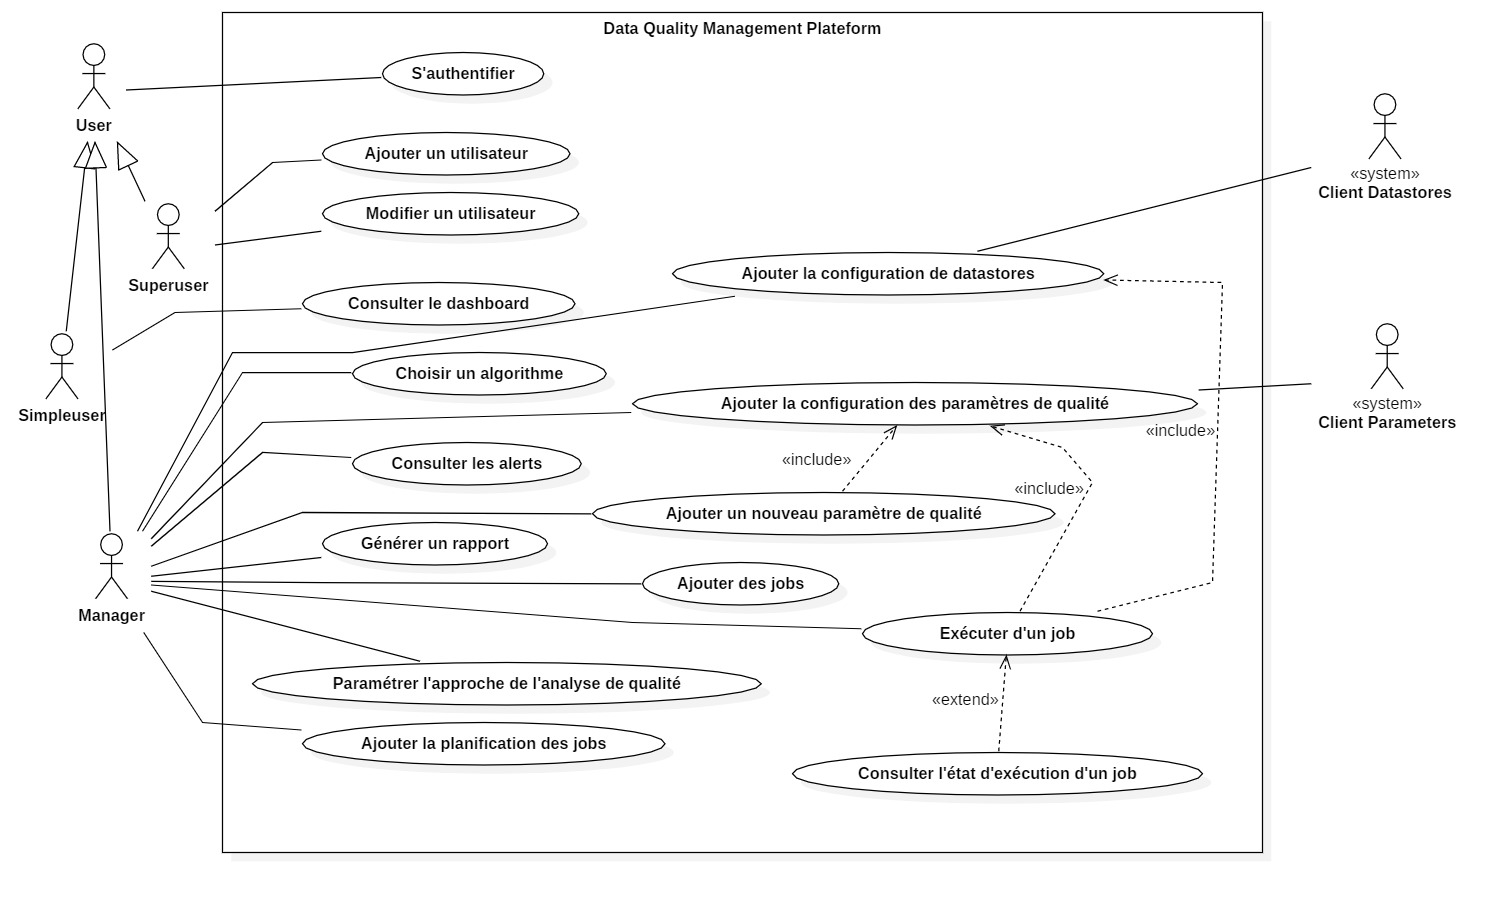
\includegraphics[width=\textwidth]{img/UseCaseDiagram.jpg}
\end{figure}


\section{Specifications techniques} 
\subsection{Les langages de développement}
Ces technologies seront utilisées pour développer cette plateforme:
\begin{itemize}
    \item \textbf{Backend} Java en utilisant Spring boot.
    \item \textbf{Frontend} Javascript en utilisant Angular.
\end{itemize}

\subsection{Les conventions de développement}
le développeur doit respecter les conventions suivantes:
\begin{itemize}
    \item \textbf{Tests:} toutes les exigences fonctionnelles doivent être testées.
    \item \textbf{SOLID:} la plate-forme doit être en conformité avec les principes SOLID.
    \item \textbf{Documentation:} la plate-forme doit offrir des documentations via Java-doc, Swagger et CompoDoc.
\end{itemize}
\end{document}